% !TeX spellcheck = da_DK
\subsection{Komparator}
\subsubsection{Teori og design}
Som nævnt i afsnit \ref{Komparatorafsnit} på side \pageref{Komparatorafsnit} anvendes en komparator til at sammenligne to inputspændinger. Der vil blive anvendt flere komparatorer og i dette tilfælde vil komparatorernes output blive tilkoblet en LED-diode eller vibrator, en modstand og den positive spændingsforsyning ($+V_{cc}$). I komparatorernes ikke-inverterende terminaler skal outputtet fra forrige blok tilsluttes. Inputtet til de inverterende terminaler skal fungere som referencespænding, hvilket anvendes til at forsyne med de beregnede tærskelværdier. Komparatorerne kan derfor have to forskellige outputs afhængig af inputspændingen. Hvis inputsignalet ligger udenfor de beregnede tærskelværdier, vil outputtet være $0V$, og dioderne og vibratoren vil ikke aktiveres. Er inputtet indenfor de beregnede tærskelværdier, vil outputtet svare til jord, da strømmen fra $+V_{cc}$ vil løbe igennem komparatorerne og derefter til jord. Derved opnås et spændingsfald over den positive (anode) og negative (katode) pol for LED-dioden og vibratoren på en værdi, der ligger over det minimale spændingsfald, der kræves for en aktivering. LED-dioderne og vibratorerne vil derved blive aktiveret og give feedback til patienten. \\

\noindent\textbf{Visuel komparator kredsløb} \\
Til den visuelle del af komparatorkredsløbet anvendes LED-dioder. LED-diodernes katode tilkobles komparatorens output, imens anoden tilkobles $+V_{cc}$. Jævnfør kravspecifikationerne i afsnit \ref{KomparatorAfs}, side \pageref{KomparatorAfs} er der valgt fem forskellige stadier for aktivering af LED-dioderne. For aktivering af LED-dioderne vil der blive anvendt otte komparatorer, da det første stadie, indeholdende den grønne LED-diode, både har en positiv og negativ tærskelværdi og derfor kræver to komparatorer. Tærskelværdierne kan både implemeteres som to spændingstræer eller som otte spændingsdelere og der er fordele og ulemper ved begge metoder. Der anvendes her otte spændingsdelere, hvor fire indgår i to vindues-komparatorer og fire almindelige komparatorer. Dette design vælges til fordel for to spændingtræer, da modstandene i et spændingstræ påvirker hinanden, hvilket kan ændre tærskelværdierne, hvis én af modstandene ikke fungerer ideelt. For at modvirke dette, anvendes en spændingsdeler for hver tærskelværdi, der fremgår af figur \figref{fig:komparator_visuel}. Konfigurationen indeholder en spændingsreference $+V_{ref}$ på $2.5$V og seks modstande (R$15$-R$20$) mellem LED-dioderne og $+V_{cc}$ for at beskytte LED-dioderne mod for høj strømstyrke og at batteriet ikke drænes. Der udarbejdes et vindues-konfigurationen som placeres for LED-dioderne (D$3$ - D$4$) ved hver af de to komparatorer (LM$311$). \textcolor{red}{Dette gøres for at adskille de to komparatorerer, så de ikke påvirker hinanden og vindues-komparatoren fungerer som ønsket.}  
\begin{figure}[H]
	\centering
	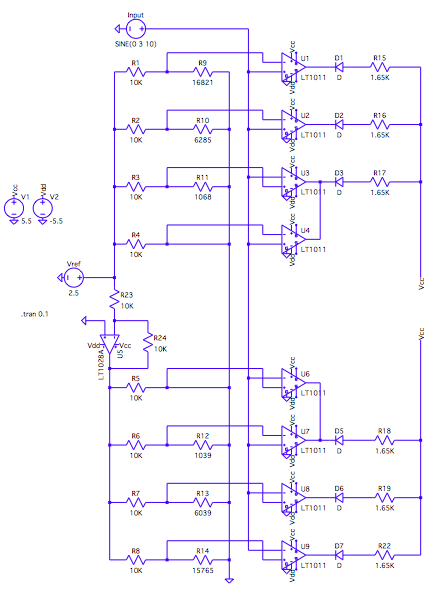
\includegraphics[scale=1.0]{figures/cProblemloesning/komparator_visuel1.PNG}
	\caption{Figuren illustrerer komparatorkonfigurationen for den visuelle del. Kredsløbet består af to dele; en for hældning i positiv retning og en for hældning i negativ retning. Hver del består af en vindues-komparator og to almindelige komparatorer. Der er implementeret en inverterende forstærker for at gøre referencespændingen negativ, så hældning i den negative retning kan dedekteres. Kredsløbet er udarbejdet i LTspice.}
	\label{fig:komparator_visuel}
\end{figure}

%%%%%%%%%%%%%%%%%%%%%%%%%%%%%%%%%%%%%%%%%%%%%%%%%%%%%%%%%%%%%%%

\noindent\textbf{Beregning af tærskelværdier og tilhørende R$1$-R$14$ modstande for aktivering af LED-dioder} \\
Inputsignalet fra forrige blok, tilpasningsblokken, ligger mellem -$2.9417$V og $3.0151$V jævnfør afsnit \ref{KomparatorAfs}, side\pageref{KomparatorAfs}. Jævnfør systemets funktionelle krav afsnit \ref{FunkKrav}, side \pageref{FunkKrav} ønskes det, at de enkelte LED-dioder skal lyse ved bestemte kropshældninger, dvs. ved en bestemt tærskelværdi. %Disse tærskelværdier sættes ud fra to punkter; det maksimale teoretiske signal  ved $25^{\circ}$ $4.0662$, og en tilgængelig spændingsreference, der kan sørge for en fast spænding til spændingstræet. 
Tærskelværdierne er udregnet til at være:

\begin{itemize}
\item $2^{\circ}$ = $0.2412$V
\item -$2^{\circ}$ = -$0.2353$V
\item $8^{\circ}$ = $0.9648$V
\item -$8^{\circ}$ = -$0.9413$V
\item $13^{\circ}$ = $1.5679$V
\item -$13^{\circ}$ = -$1.5297$V
\item $25^{\circ}$ = $3.0151$V
\item -$25^{\circ}$ = -$2.9417$V
\end{itemize}

\begin{figure}[H]
	\centering
	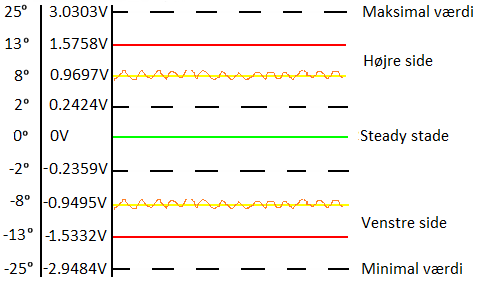
\includegraphics[scale=1.0]{figures/cProblemloesning/Taerskelvaerdier.PNG}
	\caption{Af figuren fremgår de beregnede tærskelværdier.}
	\label{fig:taerskelvaerdier}
\end{figure}

Der vælges en  spændingsreference, som består af en regulator så den kan levere $2.5$V til komparatorkredløbet. Spændingsreferencen indgår som del af en spændingsdeler og benyttes for at holde en fast referencespænding, da spændingen ved anvendelse af et batteri vil falde som funktion af tid. For at muliggøre anvendelsen af spændingsforsyningen på $2.5$V til negative tærskelværider benyttes en inverterende forstærker med et gain på $1$, der fremgår af figur \figref{fig:komparator_visuel}. Ved denne konfiguration vendes signalet uden at blive forstærket og kan på denne måde benyttes som referencespænding til negative inputspændinger.  
Når referencespændingen er kendt kan modstandene i spændingsdeleren bestemmes. Da kredsløbet trækker strøm har modstandene (R$15$-R$20$) til formål at sikre, at spændingsforsyningen ikke drænes. Hvis modstanden er høj, vil strømmen til kredsløbet være lav, og batterierne i spændingsreferencen vil derved holde længere.

Der anvendes otte spændingsdelere, hvor fire indgår som vindues-komparatorer og de resterende som almindelige komparatorer, hvillket fremgår af figur \figref{fig:komparator_visuel}.. 
For at opstille spændingsdelerne skal R$1$-R$14$ bestemmes så LED-dioderne lyser ved de ønskede tærskelværdier. For at modstandene kan bestemmes defineres R$1$ til en bestemt værdi, der her fastsættes til at være $10$K$\Omega$. Den samme værdi er gældende for R$2$-R$8$, eftersom der anvendes en spændingsdeler for hver tærskelværdi. Herefter kan R$9$-R$14$ udregnes vha. den generelle formel for en spændingsdeler jævnført \eqref{Spaendingsdeler}. Hvor følgende er kendt:
\begin{itemize}
\item $V_out$ = den ønskede tærskelværdi
\item $V_in$ = spændingsreferencen
\item R$1$-R$8$ = $10$K$\Omega$
\end{itemize}

Dette medfører at R$9$-R$14$ giver følgende resultater:\\
R$9$ = $16821\Omega$ \\
R$10$ = $6285\Omega$ \\
R$11$ = $1068\Omega$ \\
R$12$ = $1039\Omega$ \\
R$13$ = $6039\Omega$ \\
R$14$ = $15765\Omega$ \\

%%%%%%%%%%%%%%%%%%%%%%%%%%%%%%%%%%%%%%%%%%%%%%%%%%%%%%%%

\noindent\textbf{Beregning af R$15$-R$20$ modstande for aktivering af LED-dioder} \\
Jænvfør kravspecifikationerne i afsnit \ref{KomparatorAfs}, side \pageref{KomparatorAfs} for komparatoren skal forsyningsspændingen være $5.5$V. De anvendte LED-dioder i systemet er: to grønne L-$53$LG $5$mm (D$3$ og D$4$), to røde L-$53$LI $5$mm (D$1$ og D$6$) og to gule L-$53$LY $5$mm (D$2$ og D$5$). Disse LED-dioder kræver en minimum spænding på 2mA for at lyse og spændingsfaldet over LED-dioderne ligger maksimalt i intervallet $2.0$V til $2.2$ V (rød: $2.0$, gul: $2.1$ og grøn: $2.2$), men typisk mellem $1.7$V-$1.9$V. LED-dioderne skal derudover forsynes med $2$mA for at fungere, men kan forsynes med op til $150$mA, før de brændes af. LED-dioderne forsynes af en $5.5$V spændingsforsyning og tilkobles, som sagt, tilhørende modstande for bla. at undgå at LED-dioderne brænder af. Spændingsfaldet over dioderne samt den spænding LED-dioderne som minimum skal bruge for at lyse er kendte værdier, dvs. modstandene R$15$-R$20$ kan derfor findes vha. Ohms lov. Nedestående udregning giver en værdi af modstandene, hvis spændingsforsyningen giver $5.5$V til kredløbet og hvor der tages udgangspunkt i den minimale strøm for LED-dioderne:

\begin{equation}
R = \dfrac{5.5V - 2.2V}{2mA} = 1650\Omega
\end{equation}
\noindent Dermed sættes modstandene R$15$-R$20$ alle til $1650\Omega$ for at sikre, at der er tilstrækkeligt med strøm i kredsløbet til at dioderne kan lyse, uden at de brændes af eller at batterierne drænes. Opsætningen af LED-dioderne fremgår af figur \figref{fig:komparator_visuel}.

%%%%%%%%%%%%%%%%%%%%%%%%%%%%%%%%%%%%%%%%%%%%%%%%%%%%%%%%%%%
\noindent\textbf{Beregning af tærskelværdier og tilhørende R1-R5 modstande for aktivering af  vibratorerne} \\
Jævnfør kravsspecifikationerne i afsnit \ref{KomparatorAfs}, side \pageref{KomparatorAfs} skal vibratorerne have to tærskelværdier. For aktivering af vibratorerne anvendes derfor to komparatorer. Vibratorernes tærskelværdier konstrueres ligeledes vha. to parallelforbundede modstande og spændingsreferencer, samt de resterende modstande mellem vibratorerne og $+V_{cc}$. På figur X vises konstruktionen af kredsløbet med de to vibratorer og tilhørende modstande. \\

indsæt billede og word dokument \\

\noindent\textbf{Beregning af R6-R10 modstande for aktivering af vibratorerne} \\
Vibratorerne der anvendes i systemet er af typen XX... Afsnit skal skrives, når vi har information om vibratorer.  \\

FÅ SWITCH MED IND I DET? \\

\subsubsection{Simulering}
\noindent\textbf{Simulering af visuel komparatorkonfiguration} \\
Til simulering af den visuelle komparatorkonfiguration anvendes komparatorer af typen LT$1011$, da operationsforstærkerne til det reelle kredsløb er af denne type. For at udføre en simulering af den visuelle komparatorkonfiguration tilkobles kredsløbet et sinus-signal, der svinger mellem $\pm3$V. Dette gøres for at simulere signalet, der kommer fra den forrige blok, hvor arbejdsområdet er på $\pm3$V. Under simuleringen i LTspice testes det, hvorvidt den visuelle komparatorkonfiguration opfylder de opstillede specifikke krav, jævnfør kravspecifikationerne i afsnit \ref{KomparatorAfs}, side \pageref{KomparatorAfs}. Simuleringen af den visuelle komparatorkonfiguration fremgår af figur \figref{fig:komparator_visuel_simulering_samlet}. \fxnote{Vi kan starte med at simulere tærskelværdier og derefter hvordan komparatoren fungerer.}
\begin{figure}[H]
	\centering
	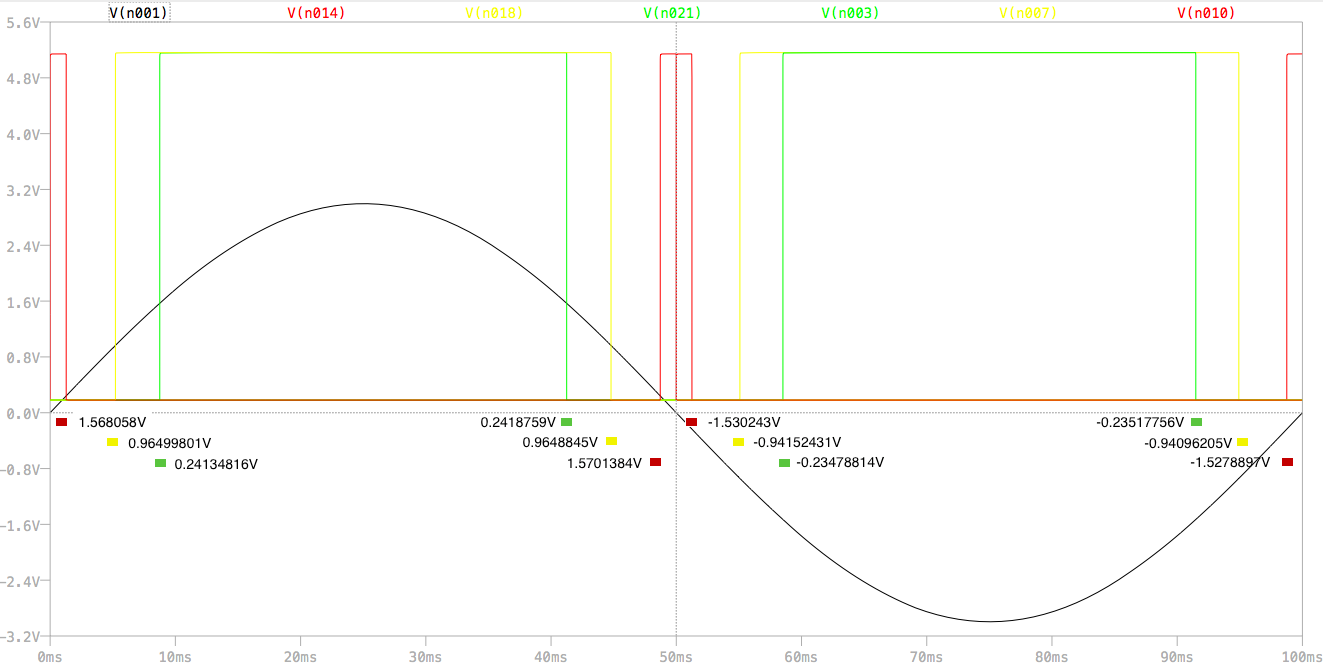
\includegraphics[scale=1.0]{figures/cProblemloesning/komparator_visuel_simulering_samlet1.PNG}
	\caption{Figuren viser simuleringen af den visuelle komparatorkonfiguration. Den sorte kurve er et sinus signal, der illustrerer blokkens inputsignal. De resterende kurver er de enkelte komparatorer, som under tærskelværdien er i negativ mætning. De røde kurver symboliserer den røde diode, de gule kurver de gule dioder og de grønne kurver de grønne dioder. Når inputsignalet når de definerede tærskelværdier, vil kurverne gå i positiv mætning og LED-dioderne vil lyse. Ved vindue-komparatoren er den positive og negative mætning ikke så høj, som ved de normale komparatorer. Dette skyldes, at signalet skal passere yderligere to LED-dioder, hvilket giver et spændingsfald. Kredsløbet er simuleret i LTspice.}
	\label{fig:komparator_visuel_simulering_samlet}
\end{figure}
På figur \figref{fig:komparator_visuel_simulering_samlet} fremgår det, at ved de enkelte tærskelværdier går signalet i positiv mætning, hvilket får LED-dioderne til at lyse. Mætningen er under $5.5$V som er den spænding LED-dioderne maksimalt kan forsynes med  \fxnote{Kontrollere af denne værdi (5.5) er rigtig}, men samtidig nok til at få dioderne til at lyse, hvilket krævede mellem $1.7-1.9$V og $2$mA. 

\begin{table}[H]
	\centering
	\begin{tabular}{|l|l|l|l|l|l|}
		\hline
					& \textit{Tærskelværdier} 	& \textit{Måling til højre} & \textbf{Måling til venstre}		&  \textit{Afvigelse for højre}  \textit{Afvigelse for venstre}\\ \hline
\textbf{$2^{\circ}$} 		& $0.2412$V  				&$0.24134816$V 			&$0.24118759$V		& $0.06\%$  &$0.005\%$ \\ \hline
\textbf{-$2^{\circ}$} 		&-$0.2353$V 					&-$0.23478814$V 			&-$0.23517756$V  	& $0.2\%$	&$0.05\%$\\ \hline
 \textbf{$8^{\circ}$} 		&$0.9648$V					&$0.96499801$V			&$0.9648845$V		& $0.02\%$	&$0.009\%$\\ \hline
\textbf{-$8^{\circ}$} 		&-$0.9413$V					&-$0.94152431$V 			&-$0.94096205$V		& $0.02\%$	&$0.04\%$\\ \hline 		
\textbf{$13^{\circ}$} 		&$1.5679$V 					&$1.5680858$V 		  	&$1.5701384$V		& $0.01\%$	&$0.14\%$\\ \hline
\textbf{-$13^{\circ}$} 		&-$1.5297$VV 				&-$1.530243$V		   	&-$1.5278897$V		& $0.04\%$	&$0.12\%$ \\ \hline
	\end{tabular}
	\caption{I tabellen ses der, at de anvendte tærskelværdier afviger fra den teoretiske værdi, hvilket er forventet af reelle komponenter. Det er en acceptabel afvigelse, så tærskelværdierne kan derfor anvendes til implementering}
	\label{Tab:Maalingtearskelvaerdier}
\end{table}

Det kan udfra \ref{Tab:Maalingtearskelvaerdier} konkluderes at afvigelsen fra de udregnede tærkselværdier stemmer overens med tolerance for tærkselværdierne jævnfør afsnit \ref{KomparatorAfs}, side \pageref{KomparatorAfs} som var på $\pm1$\%. 

\noindent\textbf{Simulering af somasensorisk komparator kredsløb} \\

\subsubsection{Implementering og test}
